\documentclass[11pt]{article}
\usepackage[spanish,es-tabla,es-nodecimaldot,es-noshorthands]{babel}
\usepackage[utf8]{inputenc}
\usepackage[T1]{fontenc}
\usepackage{lmodern}
\usepackage[margin=2.5cm]{geometry}
\usepackage{amsmath}
\usepackage{graphicx}
\usepackage{booktabs}
\usepackage{tabularx}
\usepackage{float}
\usepackage{enumitem}
\usepackage{tikz}
\usetikzlibrary{arrows.meta, positioning, calc, babel}
\usepackage[hidelinks]{hyperref}

\setlist{itemsep=2pt, topsep=4pt}

\tikzset{
  box/.style    = {draw=black!75, semithick, rounded corners=1.5pt, align=center,
                   minimum height=1.1cm, minimum width=2.6cm, font=\footnotesize,
                   fill=white},
  shade/.style  = {box, fill=black!7},
  sig/.style    = {-{Stealth[length=2mm]}, semithick},
  dsig/.style   = {{Stealth[length=2mm]}-{Stealth[length=2mm]}, thick},
  cell/.style   = {draw=black!75, minimum height=0.55cm, minimum width=1.1cm,
                   font=\scriptsize\ttfamily, inner sep=1pt, anchor=south west},
  lab/.style    = {font=\scriptsize, midway, above},
  note/.style   = {font=\scriptsize\itshape, align=center},
  rowlab/.style = {font=\footnotesize, anchor=east},
}

\newcommand{\code}[1]{\texttt{#1}}

\title{Propuesta de solución al problema de concurrencia\\
       en la comunicación SPI de la DAQ basada en dsPIC}
\author{Haniel Ulises\\Servicio social}
\date{\today}

\begin{document}
\maketitle

\begin{abstract}
El sistema DAQ-SPI emula una tarjeta de adquisición de datos tipo Quanser
mediante un microcontrolador dsPIC33CK64MC105, un puente USB--SPI FT2232H y un
conjunto de S-Functions de Simulink. Se ha observado que la comunicación se
corrompe o se interrumpe cuando la lectura del encoder y la escritura al DAC
operan simultáneamente. En este documento se analiza el código existente, se
identifican las causas del problema y se propone un esquema de comunicación
basado en una única transferencia SPI full-duplex de longitud fija por paso de
simulación, delimitada por la señal de selección de esclavo y atendida en el
microcontrolador mediante DMA.
\end{abstract}

% ===========================================================================
\section{Descripción del sistema}

La arquitectura actual se muestra en la figura~\ref{fig:arq}. En la PC, un
modelo de Simulink utiliza tres S-Functions escritas en C++ sobre la biblioteca
libMPSSE-SPI de FTDI. La función \code{initializePic} abre el canal SPI del
FT2232H y comparte su \emph{handle}, protegido por un mutex del sistema
operativo, con las otras dos: \code{escribirPic}, que convierte un voltaje en
el intervalo $[-2.5, 2.5]$\,V a un valor de 16 bits, y \code{leerPic}, que
obtiene la posición del encoder.

El FT2232H opera como maestro SPI a 1\,MHz en modo~0. El dsPIC actúa como
esclavo en su módulo SPI1, como maestro del DAC en el módulo SPI2, y cuenta los
pulsos del encoder con el módulo QEI1. El reloj del microcontrolador es el
oscilador interno FRC de 8\,MHz sin PLL, lo que da una frecuencia de
instrucción $F_{cy} = 4$\,MHz.

\begin{figure}[tbp]
  \centering
  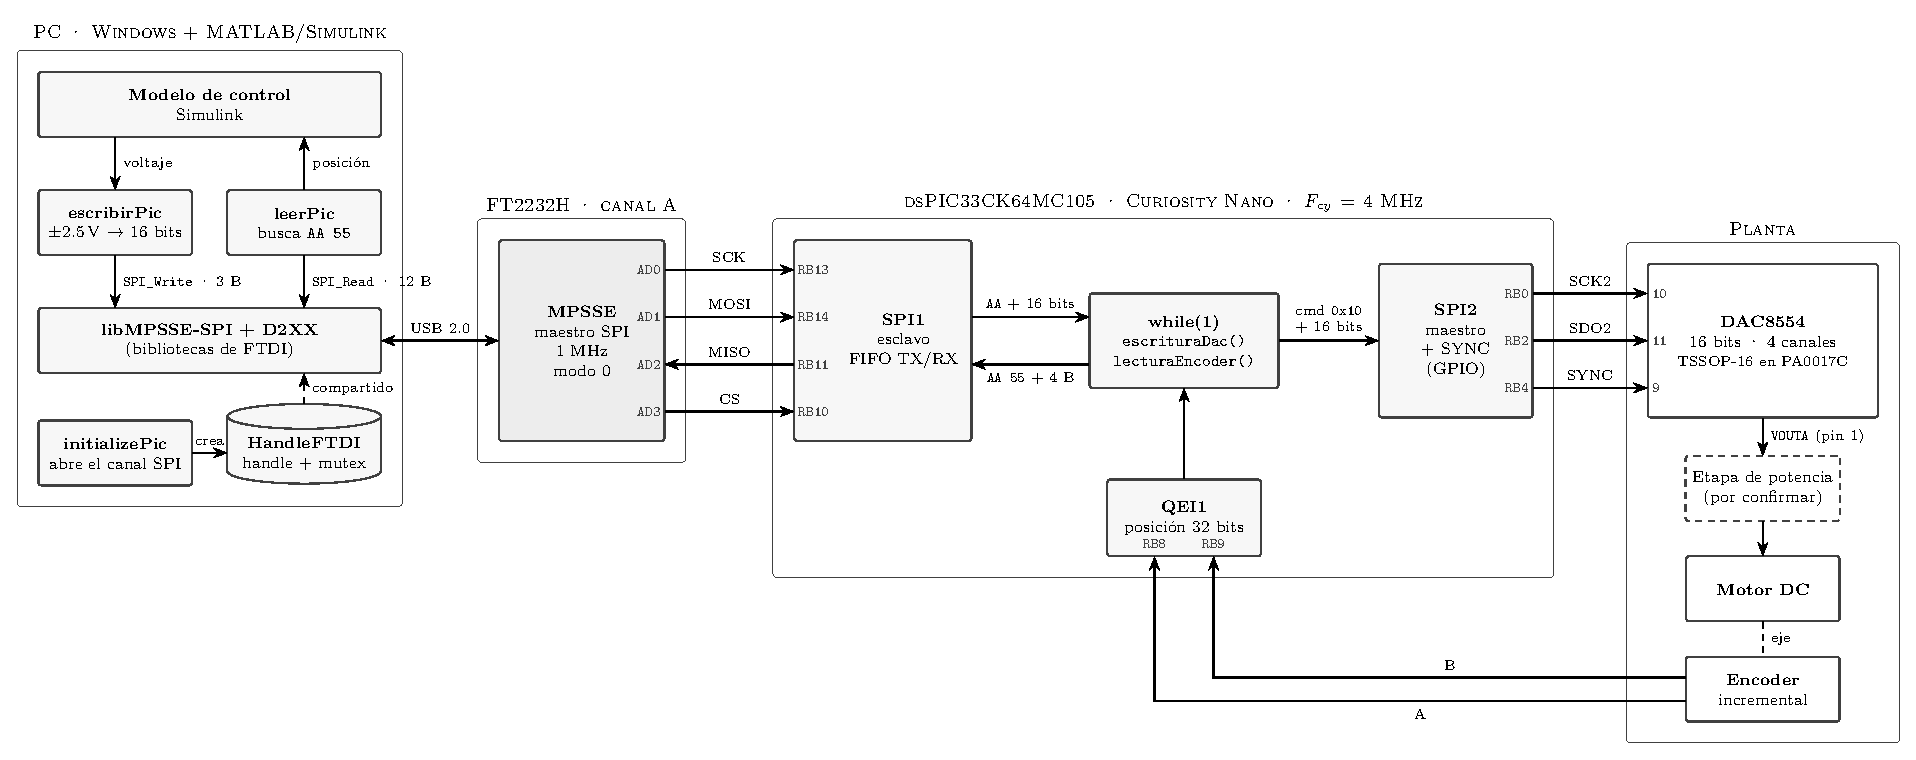
\includegraphics[width=\linewidth]{arquitectura.pdf}
  \caption{Arquitectura actual del sistema.}
  \label{fig:arq}
\end{figure}

La escritura y la lectura se realizan como transacciones independientes. Para
escribir, la PC ejecuta \code{SPI\_Write} con tres bytes: el encabezado
\code{0xAA} y el valor del DAC en dos bytes. Para leer, ejecuta
\code{SPI\_Read} de doce bytes y busca en ellos la secuencia \code{0xAA 0x55}
seguida de los cuatro bytes de la posición.

En el dsPIC, el firmware (\code{dsPicController}) consiste en un lazo infinito
que alterna dos funciones. \code{escrituraDac()} toma los bytes disponibles en
la FIFO de recepción de SPI1, reconstruye el valor mediante una máquina de
estados que busca el encabezado \code{0xAA} y lo transmite al DAC por SPI2.
\code{lecturaEncoder()} escribe seis bytes en la FIFO de transmisión de SPI1
cada vez que ésta no está llena.

% ===========================================================================
\section{Análisis del problema}

\subsection{Uso del bus como canal half-duplex}

En SPI cada pulso de reloj desplaza simultáneamente un bit en cada dirección,
de modo que toda transferencia es necesariamente de lectura y escritura a la
vez. El protocolo actual no aprovecha esta propiedad. Durante un
\code{SPI\_Write}, el dsPIC entrega por MISO bytes de su FIFO de transmisión
que la PC descarta; durante un \code{SPI\_Read}, la PC envía bytes de relleno
que ingresan a la FIFO de recepción del dsPIC como si fueran datos. Ambas
transacciones consumen o introducen bytes que el otro extremo no espera, y el
flujo de datos pierde la alineación.

\subsection{Gestión de las FIFOs en el esclavo}

De acuerdo con la hoja de datos del dsPIC33CK64MC105, la FIFO del módulo SPI
tiene una profundidad de cuatro elementos en modo de 8 bits.
\code{lecturaEncoder()} intenta escribir seis bytes, por lo que
\code{SPI1\_ByteWrite()} permanece en espera activa hasta que el maestro genere
pulsos de reloj suficientes para liberar espacio. Dado que el esclavo no
controla el reloj, el tiempo de esa espera depende por completo de la PC.

Mientras el lazo está detenido en esa espera, \code{escrituraDac()} no se
ejecuta y la FIFO de recepción, también de cuatro elementos, puede llenarse.
En ese caso el módulo activa la bandera de desbordamiento \code{SPIROV} y deja
de aceptar datos. El controlador generado por MCC no limpia esa bandera, por
lo que la recepción queda suspendida de forma permanente. Las llamadas a
\code{printf} dentro del lazo aumentan el tiempo entre lecturas y agravan la
situación.

Adicionalmente, como la FIFO de transmisión se llena sin relación con el
momento en que la PC lee, los valores de posición que recibe la PC tienen una
antigüedad indeterminada y no están alineados con el inicio de la
transacción. Por esta razón \code{leerPic} necesita buscar el encabezado
dentro de una ventana de doce bytes.

\begin{figure}[tbp]
\centering
\resizebox{\linewidth}{!}{%
\begin{tikzpicture}[x=1cm, y=1cm]
  \node[rowlab] at (-0.3,3.3) {\code{CS}};
  \node[rowlab] at (-0.3,2.3) {MOSI (PC $\to$ dsPIC)};
  \node[rowlab] at (-0.3,1.3) {MISO (dsPIC $\to$ PC)};
  \node[rowlab] at (0,0.0) {Lazo del dsPIC};

  \draw[semithick] (0,3.6) -- (0.5,3.6) -- (0.5,3.0) -- (3.8,3.0) -- (3.8,3.6)
        -- (5.5,3.6) -- (5.5,3.0) -- (12.1,3.0) -- (12.1,3.6) -- (13.2,3.6);
  \node[font=\scriptsize] at (2.15,3.85) {\code{SPI\_Write} (3 bytes)};
  \node[font=\scriptsize] at (8.8,3.85) {\code{SPI\_Read} (12 bytes)};

  \foreach \i/\t in {0/AA,1/hi,2/lo}
    \node[cell, fill=white] at (0.5+\i*1.1,2.0) {\t};
  \foreach \i/\t in {0/e2,1/e3,2/AA}
    \node[cell, fill=black!25] at (0.5+\i*1.1,1.0) {\t};
  \node[note] at (2.15,0.75) {descartados por la PC};

  \foreach \i/\t in {0/00,1/00,2/00,3/00,4/\dots,5/00}
    \node[cell, fill=black!7] at (5.5+\i*1.1,2.0) {\t};
  \foreach \i/\t in {0/55,1/e0,2/e1,3/e2,4/\dots,5/AA}
    \node[cell, fill=white] at (5.5+\i*1.1,1.0) {\t};
  \node[note] at (8.8,0.75) {datos con antigüedad indeterminada, desalineados};

  \draw[semithick, fill=black!7] (0.2,-0.5) rectangle (13.2,0.5);
  \node[font=\scriptsize, align=center] at (6.7,0.0)
    {\code{lecturaEncoder()} en espera dentro de \code{SPI1\_ByteWrite()} (FIFO de transmisión llena);\\
     \code{escrituraDac()} no se ejecuta y la FIFO de recepción no se vacía};
  \draw[sig] (12.1,2.3) -- (13.0,2.3) |- (13.6,1.3);
  \node[note, anchor=west, align=left] at (13.6,1.3)
    {FIFO de recepción llena:\\\code{SPIROV} = 1,\\la recepción se detiene};
\end{tikzpicture}}
\caption{Comportamiento del protocolo actual. Los bytes sombreados en MISO son
descartados por la PC; los bytes de relleno en MOSI ingresan a la FIFO de
recepción del dsPIC.}
\label{fig:actual}
\end{figure}

\subsection{Delimitación de tramas}

El dsPIC no utiliza la señal de selección de esclavo para identificar el
inicio y el fin de una trama; se limita a buscar el byte \code{0xAA} en el
flujo recibido. Este valor puede aparecer también dentro de los datos, y una
vez perdida la alineación no existe un mecanismo que la restablezca.

\subsection{Observaciones adicionales}

El mutex implementado en la PC impide que dos S-Functions accedan al FT2232H
al mismo tiempo, pero no interviene en ninguno de los fenómenos anteriores,
que ocurren en el uso del bus y en el firmware del esclavo. Por otra parte, al
terminar la simulación \code{initializePic} envía el valor \code{0x0000}, que
con la conversión empleada corresponde a $-2.5$\,V y no a 0\,V; el motor queda
energizado después de detener el modelo.

% ===========================================================================
\section{Solución propuesta}

La propuesta consiste en realizar una sola transferencia full-duplex de
longitud fija en cada paso de simulación, mediante la función
\code{SPI\_ReadWrite} de libMPSSE. En esa transferencia la PC envía el valor
del DAC y, simultáneamente, recibe la posición del encoder. La señal de
selección de esclavo delimita cada trama: el dsPIC procesa la trama recibida
cuando la señal regresa a nivel alto y prepara la respuesta siguiente antes de
la próxima transferencia. El movimiento de datos entre la memoria y el módulo
SPI1 lo realiza el controlador DMA, de manera que el programa principal nunca
espera al maestro. Este esquema corresponde al de una tarjeta de adquisición
comercial, en la que cada paso de simulación ejecuta una lectura y una
escritura de forma atómica.

\subsection{Formato de trama}

Ambas direcciones utilizan tramas de ocho bytes, descritas en la
tabla~\ref{tab:trama}. El número de secuencia y el código de redundancia
cíclica permiten a la PC detectar tramas corruptas o perdidas y descartarlas
en lugar de interpretarlas como datos válidos. Se conserva la conversión
actual del voltaje, $\text{valor} = 13107\,(V + 2.5)$, de modo que el valor
32767 corresponde a 0\,V.

\begin{table}[tbp]
\centering
\small
\begin{tabular}{@{}cll|ll@{}}
\toprule
Byte & \multicolumn{2}{l|}{PC $\to$ dsPIC (MOSI)} & \multicolumn{2}{l}{dsPIC $\to$ PC (MISO)} \\ \midrule
0   & \code{0xA5}   & inicio de trama              & \code{0x5A}   & inicio de trama \\
1   & \code{seq}    & número de secuencia          & \code{seq}    & eco de la última trama válida \\
2   & \code{dac\_h} & valor del DAC, byte alto     & \code{enc0}   & posición del encoder \\
3   & \code{dac\_l} & valor del DAC, byte bajo     & \code{enc1}   & (entero de 32 bits \\
4   & \code{flags}  & banderas de control          & \code{enc2}   & con signo, \\
5   & ---           & reservado                    & \code{enc3}   & \emph{little-endian}) \\
6   & ---           & reservado                    & \code{status} & estado del dsPIC \\
7   & \code{crc}    & CRC-8 de los bytes 0 a 6     & \code{crc}    & CRC-8 de los bytes 0 a 6 \\
\bottomrule
\end{tabular}
\caption{Formato de trama propuesto. El CRC-8 utiliza el polinomio \code{0x07}.}
\label{tab:trama}
\end{table}

El byte \code{flags} contiene, en su bit~0, la habilitación de la salida
analógica (con valor cero el DAC se lleva a 0\,V) y, en su bit~1, la orden de
poner en cero el contador del encoder. El byte \code{status} indica en sus
bits~0, 1, 2 y~3, respectivamente, si la última trama recibida tuvo error de
CRC, si tuvo un encabezado inválido, si se activó el temporizador de vigilancia
y si la trama no tuvo exactamente ocho bytes.

\subsection{Temporización}

La figura~\ref{fig:tiempo} muestra la secuencia en un periodo de muestreo. A
1\,MHz, la transferencia de ocho bytes dura aproximadamente 64\,$\mu$s. La
respuesta enviada en la transferencia $k$ contiene la posición muestreada al
término de la transferencia $k-1$, por lo que el dato tiene, a lo sumo, un
periodo de antigüedad. Este retardo es conocido y constante, a diferencia del
esquema actual, y debe considerarse en el diseño del controlador.

\begin{figure}[tbp]
\centering
\resizebox{\linewidth}{!}{%
\begin{tikzpicture}[x=1cm, y=1cm]
  \node[rowlab] at (-0.3,4.3) {Paso de Simulink};
  \node[rowlab] at (-0.3,3.3) {\code{CS}};
  \node[rowlab] at (-0.3,2.3) {MOSI};
  \node[rowlab] at (-0.3,1.3) {MISO};
  \node[rowlab] at (-0.3,0.3) {dsPIC};

  \draw[semithick, fill=black!7] (0,4.0) rectangle (0.9,4.6);
  \node[font=\scriptsize] at (0.45,4.3) {$k$};
  \draw[semithick, fill=black!7] (14.0,4.0) rectangle (14.9,4.6);
  \node[font=\scriptsize] at (14.45,4.3) {$k{+}1$};

  \draw[semithick] (0,3.6) -- (1.0,3.6) -- (1.0,3.0) -- (9.8,3.0) -- (9.8,3.6)
        -- (14.9,3.6) -- (14.9,3.0) -- (15.5,3.0);

  \foreach \i/\t in {0/A5,1/seq,2/dac\_h,3/dac\_l,4/flags,5/--,6/--,7/crc}
    \node[cell, fill=white] at (1.0+\i*1.1,2.0) {\t};
  \foreach \i/\t in {0/5A,1/seq,2/enc0,3/enc1,4/enc2,5/enc3,6/status,7/crc}
    \node[cell, fill=black!7] at (1.0+\i*1.1,1.0) {\t};

  \draw[semithick, fill=white] (1.0,0.0) rectangle (9.8,0.6);
  \node[font=\scriptsize] at (5.4,0.3) {transferencia por DMA};
  \draw[semithick, fill=black!20] (9.8,0.0) rectangle (11.6,0.6);
  \node[font=\scriptsize] at (10.7,0.3) {ISR};
  \draw[semithick, fill=black!7] (11.6,0.0) rectangle (13.6,0.6);
  \node[font=\scriptsize] at (12.6,0.3) {DAC (SPI2)};

  \draw[{Stealth}-{Stealth}] (1.0,-0.4) -- node[below, font=\scriptsize] {$\approx 64\,\mu$s} (9.8,-0.4);
  \draw[{Stealth}-{Stealth}] (0,5.0) -- node[above, font=\scriptsize] {$T_s$} (14.0,5.0);
  \draw[densely dashed, black!50] (0,-0.1) -- (0,5.0);
  \draw[densely dashed, black!50] (14.0,-0.1) -- (14.0,5.0);
\end{tikzpicture}}
\caption{Secuencia en un periodo de muestreo. La interrupción asociada al
flanco de subida de \code{CS} procesa la trama y prepara la respuesta antes de
la siguiente transferencia.}
\label{fig:tiempo}
\end{figure}

\subsection{Firmware del dsPIC}

La organización propuesta del firmware se muestra en la figura~\ref{fig:fw}.
Dos canales del controlador DMA atienden el módulo SPI1: uno transfiere el
buffer de respuesta \code{tx\_buf} hacia el registro de transmisión y otro
copia los datos recibidos en \code{rx\_buf}. El flanco de subida de la señal
de selección, conectada a RB10, genera una interrupción por cambio de nivel.

\begin{figure}[tbp]
\centering
\resizebox{\linewidth}{!}{%
\begin{tikzpicture}
  \node[shade, minimum height=3.2cm] (ft) at (0,1.5) {FT2232H\\maestro SPI};
  \node[box, minimum height=3.2cm] (spi1) at (4.4,1.5) {SPI1\\esclavo};
  \node[box] (dtx) at (8.6,2.8) {DMA0 (TX)\\\code{tx\_buf[8]}};
  \node[box] (drx) at (8.6,0.2) {DMA1 (RX)\\\code{rx\_buf[8]}};
  \node[shade, minimum height=1.6cm] (isr) at (13.2,1.5)
    {Interrupción de\\fin de trama\\(flanco de \code{CS})};
  \node[box] (qei) at (13.2,4.4) {QEI1};
  \node[box] (tmr) at (18.4,4.4) {Temporizador\\de vigilancia};
  \node[box, minimum height=1.6cm] (loop) at (18.4,1.5) {Programa\\principal};
  \node[box] (spi2) at (22.4,1.5) {SPI2\\maestro};
  \node[shade] (dac) at (26.0,1.5) {DAC};

  \draw[dsig] (ft) -- node[lab] {SPI} (spi1);
  \draw[sig] (dtx.west) -- ($(spi1.east)+(0,0.8)$);
  \draw[sig] ($(spi1.east)+(0,-0.8)$) -- (drx.west);
  \draw[sig, densely dashed] (isr.north west) -- node[lab, above, sloped] {prepara} (dtx.east);
  \draw[sig, densely dashed] (drx.east) -- node[lab, below, sloped] {valida} (isr.south west);
  \draw[sig] (qei) -- node[right, font=\scriptsize] {posición} (isr);
  \draw[sig] (isr) -- node[lab] {valor del DAC} (loop);
  \draw[sig] (tmr) -- (loop);
  \draw[sig] (loop) -- (spi2);
  \draw[sig] (spi2) -- (dac);
  \draw[sig] (ft.south) -- ++(0,-1.4) -| node[pos=0.25, below, font=\scriptsize] {\code{CS} (RB10)} (isr.south);
\end{tikzpicture}}
\caption{Organización propuesta del firmware. Solo el DMA y la interrupción de
fin de trama acceden a SPI1; el programa principal utiliza únicamente SPI2.}
\label{fig:fw}
\end{figure}

En la interrupción de fin de trama se verifica el encabezado y el CRC de
\code{rx\_buf}; si son correctos, se almacenan el valor del DAC y las banderas
y se actualiza el número de secuencia, y en caso contrario se registra el
error en \code{status}. A continuación se deshabilita y se vuelve a habilitar
el módulo SPI1. Según la hoja de datos, la deshabilitación reinicia el módulo,
con lo que se vacían las FIFOs y se borra cualquier condición de
desbordamiento; así cada trama comienza alineada aunque la anterior haya
fallado. Después se lee el contador del QEI, se construye en \code{tx\_buf} la
respuesta con su CRC y se reprograman ambos canales de DMA. Finalmente se
reinicia el temporizador de vigilancia y se indica al programa principal que
hay un valor nuevo para el DAC.

El programa principal se limita a transmitir al DAC, por SPI2, los valores
nuevos que reporta la interrupción. Al tratarse de un periférico distinto, esta
operación no interfiere con la comunicación con la PC. El temporizador de
vigilancia lleva el DAC a 0\,V si transcurren 50\,ms sin recibir una trama
válida, de forma análoga al comportamiento de una tarjeta comercial ante la
pérdida de comunicación. Se eliminan además las llamadas a \code{printf}. El
esquema es viable con la frecuencia de reloj actual, ya que el DMA no depende
de la velocidad de la CPU; si se requiere mayor margen para la interrupción,
puede habilitarse el PLL.

\subsection{Software en la PC}

Se propone conservar \code{initializePic} y sustituir \code{leerPic} y
\code{escribirPic} por un único bloque que reciba el voltaje deseado y entregue
la posición del encoder junto con un contador de errores de comunicación. Al
existir un solo bloque que accede al FT2232H, el mutex deja de ser necesario.
El bloque ejecutará \code{SPI\_ReadWrite}, disponible en la versión de
libMPSSE incluida en el repositorio, manteniendo activa la señal de selección
durante toda la trama. Su periodo de muestreo será fijo, por ejemplo de 1\,ms,
en lugar de heredado. Cuando una trama resulte inválida, el bloque conservará
la última posición válida e incrementará el contador de errores. Al terminar la
simulación se enviará una trama con el valor 32767 y la salida deshabilitada.

\subsection{Correspondencia con los problemas identificados}

\begin{table}[tbp]
\centering
\small
\begin{tabularx}{\linewidth}{@{}p{4.2cm}X@{}}
\toprule
Problema & Tratamiento en la propuesta \\ \midrule
Uso half-duplex del bus & Una transferencia full-duplex por paso; ningún byte se descarta. \\
Respuesta sin sincronía con el maestro & La respuesta se construye al terminar cada trama y se transmite completa en la siguiente. \\
Espera activa en el lazo principal & El DMA realiza la transferencia; el programa principal no accede a SPI1. \\
Desbordamiento sin recuperación & El DMA vacía la recepción al ritmo del bus y SPI1 se reinicia en cada trama. \\
Falta de delimitación de tramas & La señal \code{CS} marca el inicio y el fin de cada trama; el CRC detecta corrupción. \\
Valor de reposo incorrecto & Se envía 32767 (0\,V) al terminar; el temporizador de vigilancia cubre fallas de comunicación. \\
\bottomrule
\end{tabularx}
\caption{Correspondencia entre los problemas identificados y la solución propuesta.}
\end{table}

% ===========================================================================
\section{Validación y plan de trabajo}

La implementación se realizará en cuatro etapas. En la primera se desarrollará
el nuevo firmware a partir de \code{dsPicController}. En la segunda se
escribirá un programa de prueba en la PC, independiente de Simulink, que envíe
al menos cien mil tramas con valores conocidos y contabilice los errores de CRC
y de número de secuencia; el criterio de aceptación es la ausencia de errores.
Durante estas dos etapas se utilizará un analizador lógico sobre las señales
SCK, MOSI, MISO y \code{CS} para verificar la forma de las tramas y medir la
duración de la interrupción. En la tercera etapa se implementará el nuevo
bloque de Simulink, y en la cuarta se realizarán pruebas con el motor: una
rampa de voltaje verificada con osciloscopio y la comparación de la posición
medida contra un desplazamiento conocido. En esta etapa se medirá también el
tiempo de ida y vuelta por USB para determinar el periodo de muestreo mínimo
alcanzable.

\section{Consideraciones}

El cambio de protocolo afecta tanto al firmware como a las S-Functions, por lo
que ambas partes deben actualizarse de manera conjunta. La latencia del bus USB
y la planificación de procesos de Windows limitan el periodo de muestreo mínimo
y pueden introducir variaciones entre pasos, con independencia del firmware.
Por último, la configuración del DMA en modo esclavo es la parte más delicada
de la implementación; por ello se validará con el programa de prueba antes de
integrarla con Simulink.

\begin{thebibliography}{9}
\bibitem{ds} Microchip Technology, \emph{dsPIC33CK64MC105 Family Data Sheet},
  DS70005399D.
\bibitem{cnano} Microchip Technology, \emph{dsPIC33CK64MC105 Curiosity Nano
  User's Guide}, DS70005517.
\bibitem{mpsse} Future Technology Devices International, \emph{AN\_178: User
  Guide for libMPSSE-SPI}.
\end{thebibliography}

\end{document}
